%
\documentclass[11pt]{article}
\usepackage{amssymb}
\usepackage{amsmath}
\usepackage{amsthm}
\usepackage{pst-all}
\usepackage{newicktree}
\usepackage{graphicx}
\usepackage[left=1.4in,right=1.4in,top=1in,bottom=1in,includeheadfoot]{geometry}
\usepackage{setspace}
\usepackage{natbib}

\newtheorem{theorem}{Theorem}
\newtheorem{corr}{Corollary}
\newtheorem{assumptions}{Assumptions}
\newtheorem{definition}{Definition}

\DeclareMathOperator*{\argmax}{arg\,max} 

\frenchspacing
\linespread{1.25}
\parskip= 2 pt

\title{Foundations of the Age-Area Hypothesis \\ \large{Preliminary - Not for Citation}}
\author{\textbf{Matthew J. Baker} \\ Department of Economics \\ Hunter College and the Graduate Center, CUNY}

\begin{document}

\maketitle
\begin{abstract}
\noindent Historical mass migrations have played a seminal role in shaping the global distribution of cultures. A commonly-used tool in theorizing about the nature and origins of mass migrations is the so-called Age-Area Hypothesis advanced by \cite{sapir16}. The Age-Area hypothesis posits that the origin point of a linguistic stock or phylogeny is most likely where the languages comprising the stock are most divergent. While compelling and often corroborated, the Age-Area Hypothesis has never been founded in basic principles, and this lack of structure limits its use. I describe a micro-founded model of the Age-Area Hypothesis, and develop an Age-Area Theorem. The model allows computation of probabilities that different locations are the origin points for the constituents of a linguistic stock. The model also provides a probabilistic explanation of Occam's razor: migratory paths that are simpler in a well-defined sense explanations are also more likely. The paper concludes with applications to the origins of the Na-Dene and Afro-Asiatic Ethno-linguistic groups. 
\end{abstract}
\newpage

\section{Introduction}
Studying the impact of ethnic, genetic, and cultural diversity on economic outcomes has become a central part of economics. \cite{ashraf13}, for example, discuss the nuanced role that genetic diversity might play in driving modern economic outcomes, while \cite{spolaore09} describe the importance of genetic distance and economic distance between populations. 

As \cite{cavalli95} have pointed out, genetic, ethnic, linguistic, and cultural diversity are all closely related, and much recent economic research (reviewed in \cite{alesina05}) has focused on the relationship between ethnic diversity, fractionalization and economic growth. Some research, such as \cite{spolaore13}, develops a link between ancient institutions and cultural practices on modern economic outcomes. 

Other work has pushed this agenda in a different direction, with the aim of understanding the origins of ethnolinguistic and genetic diversity around the world.  For example, \cite{michalopoulos12} shows that geographical diversity is an important determinant of human diversity.  \cite{ahlerup12} develop a model of ethnic diversity based on genetic drift and migration. They show that, over time, populations spread out and experience cultural drift, and that populations that have been in place longer tend to be more culturally diverse. There is a long tradition of this in other disciplines, as described in \cite{mace05}. 

A - perhaps ``the'' - key contributor to the world-wide distribution of cultures are historical, large-scale mass migrations. For example, \cite[p. 144]{bellwood13}, in addition to describing the close relationship between genetic, linguistic, and archaeological evidence, writes ``...three histories of long-term language and population spread, each of vast extent, fundamentally shaped the long-term course of change across most of sub-Saharan Africa.'' 



A critical tool in understanding the timing and sequence of events behind these world-shaping mass migrations is the so-called Age-Area Hypothesis (henceforth AAH). While the exact origins of the idea are unclear, a leading early development and application of the idea is \cite{sapir16}, a study of the geographical origins of the North American Na-Dene language group. The AAH is often invoked when linguistic evidence is used to develop or support hypotheses about where groups of related  cultures originated, how they evolved over time, and how the current geographical distribution of the cultures came to be.\footnote{One must be careful in invoking ``the'' Age-Area Hypothesis. As I will elaborate below, this paper concerns what might be called the Linguistic Age-Area Hypothesis - not the related Age-Area Hypothesis that posits the wider the distribution of a cultural trait, the older it likely is.} The AAH provides a critical link between geography and linguistic phylogenies. While one can find competing and sometimes contrary definitions in the literature, briefly stated, the hypothesis says that the geographic area where a phylogeny originated is most likely the place where the component languages of the phylogeny are most divergent, or maximally differentiated.

Applications - either implicit or explicit  - abound. \cite{atkinson03}, following the original ideas in \cite{dogolpolsky88}, couple computational linguistics with the AAH to suggest that the Indo-European languages originated in Anatolia, not, as has sometimes been argued, on the steppes of Siberia. \cite{ruhlen94} uses the AAH and also provides overviews of debates about the origins of the Na-Dene cultures, the Bantu expansion in Africa, and the peopling of the South Pacific. \cite{ehret01} Makes extensive and efficient use in hit sweeping account of how and when the cultures of Africa found their current locations.

In spite of its widespread invocation, there is, to my knowledge, no theoretical basis for the hypothesis. The lack of a theoretical basis for the  AAH is a problem not only because it leads to imprecise definition, but also because it is difficult to use in technical situations. Suppose one wished to include a migratory path in a statistical model of migration and cultural evolution, or that one wanted to integrate the timing and path of migration into a larger statistical model, perhaps with an eye toward more accurately controlling for relatedness between differing peoples. Since the hypothesis has no theoretical underpinnings, it is difficult to see how to construct a likelihood for a certain path or migratory history, or even for the likelihood of competing hypotheses.

I develop a theoretical foundation for the age-area hypothesis. The model is micro-founded in the sense that it can be based on microeconomic principles and an associated back story. The theory shows how probabilities that different locations as being the point of origin and Occam's razor are interdependent. That is, it turns out that migratory histories that are simpler in a well defined sense are also more likely. The model indicates that migratory paths that originate at deeper points in a phylogenetic tree can be thought of as simpler in a very precise fashion, in that inclusion of such paths in a migratory history also results in a model with fewer parameters. These ideas also lead to a particular definition of divergence or dissimilarity for each constituent culture in the phylogeny. 

I then develop an Age-Area Theorem using these ideas. The theorem says that under some assumptions, a culture that is more linguistically divergent from the others in the stock is also more likely to be the point of origin of the stock. I then present a computational algorithm which relies upon backwards traversal of a phylogenetic tree, along with some extensions of the model. I conclude by discussing some applications. The theorem, when applied recursively, also yields what can be construed as a maximum-likelihood migratory path. 

It is worth emphasizing that the model can be used to formulate an likelihood function for migratory patterns, and hence can be included as part of a larger estimation problem. Maximum likelihood methods are commonly used in linguistics to estimate linguistic divergence times. So, using the results of this paper, one could in principle estimate or include the implied migratory path as part of a larger phylogenetic estimation problem. Likelihood methods are also amenable to Bayesian techniques, which expand estimation possibilities tremendously, and provide an avenue for including archaeological and genetic evidence in estimation as well. 

\section{Background Literature}

\citet[p.12]{trask00} attributes the (Linguistic) Age-Area Hypothesis - also called the center-of-gravity principle, the genetic diversity principle, and Sapir's principle - to the work of Latham (1851, 1862) and \cite{sapir16}. \cite{trask00} further notes that Mallory (1997) and Nichols (1997a) have employed and qualified the AAH in various ways.   \citet[p.336]{dimmendaal11} expresses some doubts about the exact origins of the AAH, referring to it as the ``principle of least effort'', and notes that ``This principle probably was applied first by the scholars working on Amerindian Languages, e.g. \cite{sapir16} and Dyen (1956)''.

In what seems to be the initial application of the idea, \cite{sapir16} writes:

\begin{quote}
 As is well known, [Athabaskan] languages are spoken in three geographically isolated areas, a very large northern area (interior of Alaska to near Hudson Bay), a Pacific area (southwestern Oregon and Northwestern California), and a southern area (Arizona, New Mexico, and western Texas)...it would seem that the historical center of gravity lies rather in the north than in either of the other two regions and that the occupation of these latter was due to a southward movement of Athabaskan-speaking tribes. It is important to observe that the argument is not in any way dependent on the fact that the northern tribes cover a much vaster territory that those of the other two groups or even directly on the fact that probably a larger number of distinct dialects are spoken in the north than elsewhere. The argument for the northern provenience of the Athabaskan tribes is clinched by a further linguistic fact, namely that the Athabaskan dialects from one of the three major divisions of the Na-dene stock, the other two being Haida and Tlingit. The fact that the latter are spoken in the northwest coast area so emphatically locates the historical center of gravity of the stock in the north that it becomes completely impossible to think of the Athabaskan tribes as having spread north from California or the southwest. 
\end{quote}



The principle that divergent dialects are a close tracer of spatial distribution of cultures has often been applied. 

As a note of caution, there are other, related ideas that are also often invoked. For example, the Sapir-Whorf Hypothesis is unrelated in that it refers to the idea that peoples' thinking is influenced by the structure of their language. What might be called the Cultural Age-Area Hypothesis is the principle that the more widely geographically distributed a cultural trait is, the older it is. 


\section{Problem Description and Motivation}

Consider the hypothetical phylogenetic tree displayed in figure \ref{fig1}. For clarity, the figure depicts the phylogenetic relationship between cultures, which has perhaps been obtained through a careful analysis of the languages of the cultures so that one can deduce the times at which the cultures seem to have separated. A is evidently the most divergent culture in that the last time at which the cultures had a common ancestor is further in the past than it is for any of B, C, D, E, all of whom are closer relatives to one another. D and E are the most closely related cultures. To avoid forming impressions based on evidence that is not part of the hypothesis, we will suppose that the locations of the
groups have been concealed from us, and that we have no access to archaeological or historical information about the constituent cultures of the phylogenetic tree came to be in their current locations.

The AAH asserts that the point of origin of the  stock was A's current location, as A is, evidently, the most divergent culture from the group.\footnote{It should be mentioned that there are competing definitions of the hypothesis.} Recursive application of the AAH would lead one to a most likely migratory route: the stock originated at A's location. There was then a migration from A's location to B's location, then from B to C, and then from C to either D or E.  

\begin{figure}
\begin{center}
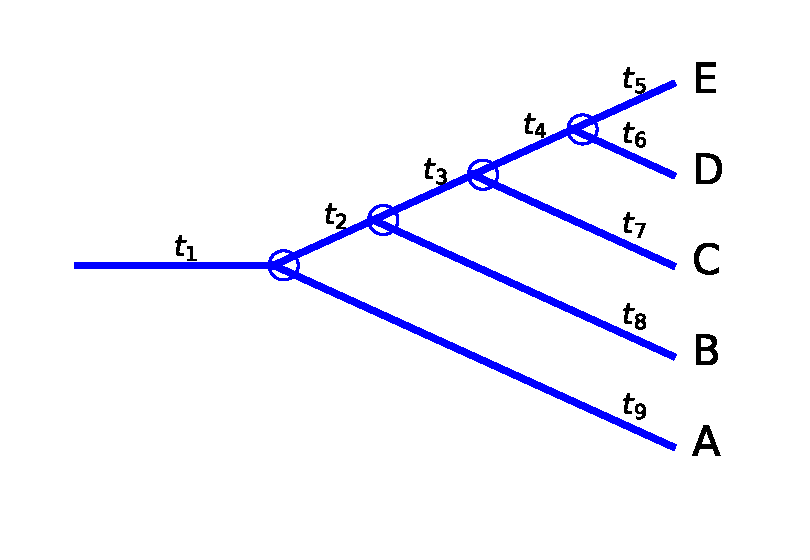
\includegraphics[width=\textwidth]{AncillaryFiles//figure1.eps}
\caption{A Phylogenetic tree} \label{fig1}
\end{center} 
\end{figure}

Why would one believe this was the most likely explanation for how the cultures came to be where they are?\ There are a number of other possible routes, even though the phylogenetic tree constrains the possibilities. For example, it can never be the case that a migration from D to E preceded one from D to C; this would be inconsistent with the observed linguistic drift over time. But another possible  sequence of migratory events would be for an initial migratory episode from C to A, followed by another from C to B, followed by yet another migration from C to D or E.

\begin{figure}
\begin{center} 
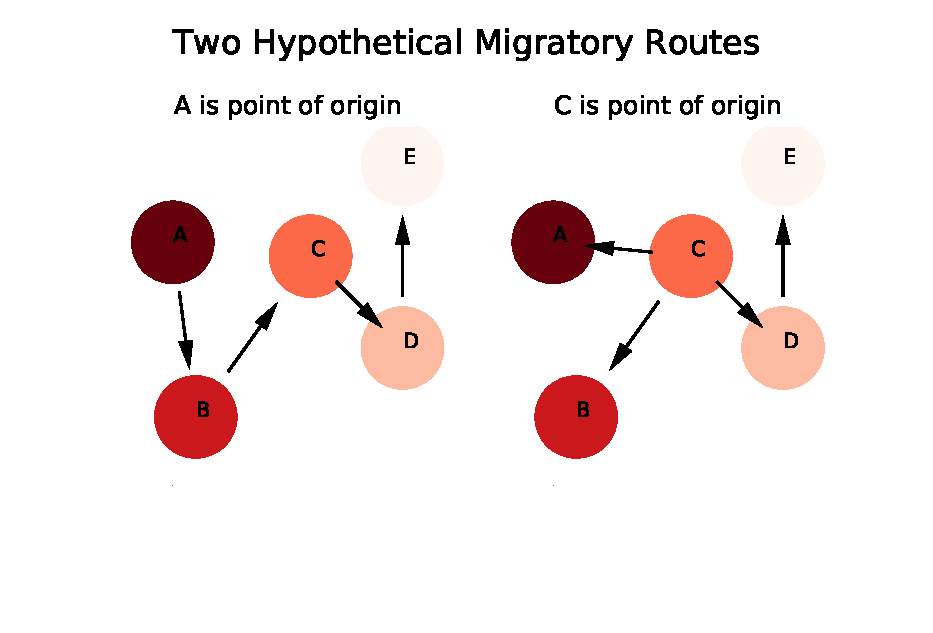
\includegraphics[width=\textwidth]{AncillaryFiles//figure2.eps} 
\caption{Potential migratory routes among a language stock consisting of five groups, following the Phylogenetic Tree in figure.} \label{fig2}
\end{center} 
\end{figure}

These two possible migratory routes are presented in figure \ref{fig2}, and the AAH asserts that the right-hand sequence is a less-likely migratory history than that on the left. Why? One might simply appeal to Occam's razor - the events on the left-hand side of figure \ref{fig2} require only one migratory chain, while the events on the right-hand side require three separate expansions: an initial migration from A to C, followed by another from A to B. A third migratory event is sufficient to take care of the last two groups: it begins from C continues to D, and then to E. We can now pose our question as follows: if we believe these migratory events to be rare, and we wish to conserve them in explaining historical migrations, what sort of model would accomplish this? But can one make this operational in a more formal setting? Can one characterize parsimony in a meaningful mathematical and probabilistic way? 

\section{A model}

\subsection{Tree Basics}

I assume throughout that the entire phylogenetic tree is known, so the universe of migratory events that needs to be explained is observed. I also assume the tree is a full, rooted, binary tree, meaning that there is a single origin node and branch, all other nodes have a single parent, all interior nodes have exactly two children, and all terminal nodes have zero children. 

A binary tree with $n$ taxa or leaves has $n-1$ internal nodes. The tree in figure \ref{fig1}, for example,  has five terminal nodes/taxa  and four internal nodes. This also applies to subtrees, which means that if a node has $k$ successors (children and childrens' children, etc.), then it is followed by $k-1$ nodes.

\subsection{Migratory Chains}
 
I build the model around what I refer to as \textit{migratory chains}. Roughly speaking, a migratory chain is a directed path from the root of the tree to an end node. I call a  collection of migratory chains that completely span the tree history a \textit{migratory history}. Hypothesizing that a particular culture or society is the point of origin of the tree amounts to positing some sequence of migratory chains through the phylogenetic tree. I assume that a migratory chain has the following properties.

\begin{assumptions}{Migratory Chains}    
\begin{enumerate}
\item Each migratory chain occupies a single location at a given point in time.
\item When a chain ``emigrates'' from its current location, a new chain starts in its place at the given location.
\item Migratory chains ``emigrate'' according to an exponential density.
\item Each migratory chain is distinct in that it has its own parameterization.
\end{enumerate}
\end{assumptions}
I will call a mass-migration history originating at location $l$ $\mathcal{H}_l$, and will assume that only mass-migration histories requiring the minimal number of events to explain the current distribution of cultures. This  means that\textit{any} history will have exactly $n-1$ migrations to span the tree. For example, the migratory events like those in figure \ref{fig2} following from the tree in figure \ref{fig1} will all have exactly 4 arrows between nodes, regardless of where they have started and how many chains are needed to explain things. Each location for our terminal nodes $l=1,2,3,\hdots L$ then will come along with a set of migratory histories $\mathcal{H}_l$. We will refer to the number of migratory chains corresponding with $\mathcal{H}_l$ as $C_l$. 

These ideas can be applied to develop a likelihood associated with any particular history, and then, using the histories, develop a measure of divergence that relates probability and divergence, which can be stated as an `Age-Area Theorem' which relates $\mathcal{H}$, $\mathcal{C}$, and $\mathcal{P}$, the probability that point $l$ is the point of origin for the locations/cultures in $L$. In this context, parsimony or Occam's razor suggests that simpler explanations - those with smaller $\mathcal{C}$'s - have higher probabilities and this is in indeed true under Assumptions 1, owing to the shape of the exponential distribution.

To preview the basic logic, I  develop a comparison of the two scenarios described in figures \ref{fig1} and \ref{fig2} within the confines of the model. I begin by assuming that we do not know the exact times at which branching events occur, but instead only know the basic structure of the tree. The points can be treated as known but can be `integrated out' by replacing the Exponential model with a Poisson model. 

The first migratory history described on figure \ref{fig2} requires an initial migratory chain to start at the root of the tree, which then proceeds from location $A$ to $B$, then from B to $C$ and then finally to $D$ or $E$.\footnote{In the next subsection, I will describe a more intricate example in which a decision must be made among multiple possibilities} But each time the migratory chain proceeds to a new location, by Assumption 1, a new one starts in its place. Importantly, in the example in figures \ref{fig1} and \ref{fig2}, these new chains never create migratory events and only lead to terminal nodes. 

Given these observations, the probability of observing this sequence of events can be written by combining the densities of the components of  $H_A$:
\begin{equation} \label{e1}
P_A = \frac{(\lambda_1 T)^4e^{-\lambda_1T}}{4!}\frac{(\lambda_2 t_6)^0e^{-\lambda_2t_6}}{0!}\frac{(\lambda_3 t_7)^0e^{-\lambda_3t_7}}{0!}\frac{(\lambda_4 t_8)^0e^{-4t_8}}{0!}
\end{equation} 
I have labelled this expression $P_A$ because it is the probability of this migratory history conditional on emanating from location $A$.

Equation (\ref{e1}) is perhaps more expansive than necessary, as all the terms raised to the $0$th power are equal to one. I have included them in the expression to illustrate that they in some sense represent degenerate migratory chains. That is, the probability in equation (\ref{e1}) could also be written as:
\begin{equation} \label{e2}
P_a = \frac{(\lambda_1 T)^4e^{-\lambda_1T}}{4!}e^{-\lambda_2t_6}e^{-\lambda_3t_7}e^{-4t_8}
\end{equation} 
The log-likelihood associated with equation (\ref{e2}) is:
\begin{equation} \label{e3}
\ln P_a  = 4\ln(\lambda_1 T) -4\lambda_1T-\ln(4!)-\lambda_2t_6-\lambda_3t_7-\lambda_4t_8
\end{equation} 
What values of $\lambda_i$ maximize the likelihood in (\ref{e3})? First, $\lambda_2=\lambda_3=\lambda_4=0$ at the optimum. Since these chains never go further than their current locations, the maximum likelihood estimate suggests that they are degenerate with rate parameter equal zero. 

The derivative of (\ref{e3}) with respect to $\lambda_1$, however, generates a meaningful parameter estimate. Differentiating with respect to $\lambda_1$ and solving the first-order condition gives $\lambda_1^*=\frac{4}{T}$. Substituting this and other optimal values back into the objective function gives the (concentrated) likelihood for $P_a$ as:
\begin{equation}  \label{l3}
P_A=\frac{4^4e^{-4}}{4!}
\end{equation}

A point of interest about equation (\ref{l3}) is that it reflects that only one non-degenerate migratory chain is needed to explain the whole tree, given that the migratory history starts at $A$. In this sense, this a parsimonious explanation for the current distribution of cultures. 

Contrast this with the case in which $C$ is posited to be the origin point of the constituent cultures of the tree. To maintain consistency with the linguistic or genetic analysis, the requirements are:  1) a migratory chain starting at $C$ leading to $A$, 2) another migratory chain starting at $C$ going to $B$, and then 3) a migratory chain that starts at $C$ and proceeds to $D$ (or $E$) and then finally to $E$ (or D). Degenerate chains start at location $C$ and $D$ (or $E$). According to the model, each of these chains requires its own Poisson/Exponential parameter, which, omitting degenerate chains, gives:
\begin{equation} \label{l4}
P_{C}=\frac{(\lambda_1t)^1e^{-\lambda_1t}}{1!}\frac{(\lambda_2(t-t_0))^1e^{-1}}{1!}
\frac{(\lambda_3(t-t_0-t_1))^2e^{-\lambda_3(t-t_0-t_1)}}{2!}
\end{equation} 
Maximizing $P_{}_{C}$ in (\ref{l4}) with respect to $\lambda_1,\lambda_2$ and $\lambda_3$, and substituting the result back into the right-hand side of (\ref{l4}) gives:
\begin{equation} \label{l5}
P_{C}=\frac{1^1e^{-}}{1!}\frac{1^{1}e^{-1}}{1!}\frac{2^2e^{-2}}{2!}=
\frac{2^2e^{-4}}{2!}
\end{equation} 

Suppose that the origin point was known to be one of these two locations. According to equation (\ref{l5}), the likelihood that $A$ is the point of origin relative to $C$ depends upon $P_A /(P_A+P_C)$; a race between the functions $\frac{4^4}{4!}$ and $\frac{2^2}{2!}$, so the relative probability  $A$ is the point of origin would then be 84\%. 

A key feature of the previous analysis is the function: 
\begin{equation*}
a(n)=\frac{n^n}{n!}
\end{equation*}
which is convex in $n$. This convexity, which owes to the structure of the Poisson-Exponential distribution, implies that one is better off with explanations that require fewer non-degenerate parameters, or, equivalently, more degenerate parameters, which have the effect of lumping migratory events into longer chains. Breaking up a migratory chain into two smaller chains eschews this convexity, and results in a less likely explanation. That is, for any  $k \in (1,n-1)$, it is true that:
\begin{equation*}
a(n) > a(n-k)a(k)
\end{equation*} 

This example illustrates the essentials of the model. The biggest detail that needs to be worked out is how migratory chains that are more parsimonious and therefore more likely relate to a measure of linguistic divergence. 

\begin{definition}{\textbf{Divergence}:}
Let $N^*$ denote the maximum number of migratory events that can be touched off from a location $l$, and let $C^*$ denote the minimum total number of non-degenerate chain migrations needed to explain all current locations if $i$ is the location of origin. Then, define the \textbf{Divergence} of language $i$ :
\begin{equation*}
D_i=\frac{N^*}{C^*}
\end{equation*}
\end{definition}


\section{ Age-Area Theorem}

\begin{theorem}[Age-Area Theorem]
Suppose that Assumptions 1 hold, and define Divergence as in definition 1. Then  
\begin{equation*}
D_i \geq D_j \Longleftrightarrow p_i\geq p_k
\end{equation*}
and in particular
\begin{equation*}
i=\argmax\left[D_1,D_2,D_3,\hdots,D_n\right] \Longleftrightarrow i=\argmax\left[p_1,p_2,p_3,\hdots,p_n\right]
\end{equation*}
\end{theorem}
\begin{proof}

Observe first that the probability that $i$ is the point of origin is a product of the functions $a$, which are convex in the number of migrations covered by a migratory chain. Thus, if $C_i$ chains are required, the length of each are $N_i$, we may write:
\begin{equation*}
p_i=\prod_{i=1}^{C_i} a(N_i)
\end{equation*} 
By the convexity of $a(N)$, breaking any chain into smaller chains, or breaking any grouping of chains into more chains reduces $p_i$.  
\end{proof} 

Of course, the measure of divergence could be constructed in many different ways so long as it is increasing in the length of the longest chain, and decreasing in the number of chains. The above-mentioned function is a measure that is easily constructed using any phylogenetic tree.  

\subsection{Additional Examples and Discussion}

Consider as an additional example the hypothetical tree described in figure \ref{ex1}.

\begin{figure}
\begin{center}
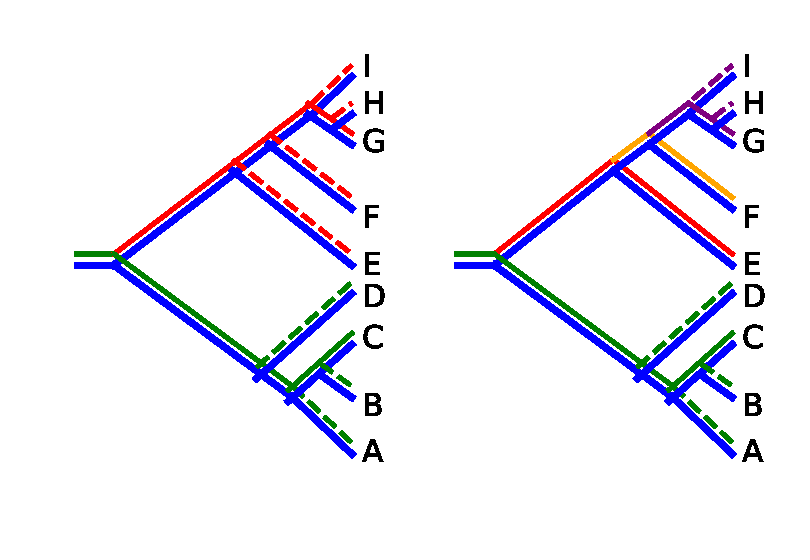
\includegraphics[width=\textwidth]{AncillaryFiles//example1.eps}
\caption{Two hypothetical migratory histories through a given Phylogenetic Tree. The picture on the left takes location $E$ as the point of origin, while that on the right takes point $I$ as the origin. } \label{ex1}
\end{center} 
\end{figure}

I have superimposed hypothetical migratory paths on figure \ref{ex1} based on different points of origin. The point of origin of the left-hand figure is posited to be point $E$, which necessitates a best migratory history with two migratory chains.  The first is one that starts at $E$ and goes to $D$'s location, and then from $D$'s location to $A$'s, from $A$'s to $B$'s, and finally from $B$'s to $C$. This history is traced out in green on the figure. A second migratory chain (traced in red) must then be invoked to explain the sequence of events leading to the upper half of the tree. This chain begins at $E$'s location again, and then moves on to $F$'s, then $I$'s, then $H$'s, and finally to $G$'s location. Under the model, the likelihood of this sequence of events is:

\begin{equation*}
P^*_E =  \frac{4^4e^{-4}}{4!}\frac{4^4e^{-4}}{4!} =\left(\rigth\frac{4^4}{4!}\right)^2e^{-8}
\end{equation*}

This reflects the two required, non-degenerate migratory chains to explain the sequence of events. 

If $I$'s location is  to be the point of origin, more migratory chains need to be invoked. The first chain is again traced out in green, mimicking the case in which $E$ is the point of origin. But to explain how a group got to point $E$ given $I$ was the starting point, we need a single migratory chain consisting of a sole migratory event. We also need another migratory chain to explain how a group got to point $F$. Finally, a fourth migratory chain going from $I$, and then to $H$, and finally on to $G$ is needed. The likelihood of these events is then:

\begin{equation*}
P^*_I =\frac{4^4e^{-4}}{4!}\frac{1^1e^{-1}}{1!}\frac{1^e^{-1}}{1!}\frac{2^2e^{-2}}{2!}=\frac{4^4}{4!}\frac{2^2}{2!}e^{-8}
\end{equation*} 

So, once again, we see the role that convexity and degeneracy plays in driving differences in likelihood. If we were to compare the probability of these two locations to get a relative likelihood, we get $P^*_E/(P^*_I+P^*_E)
=.84.

One issue that has been masked so far is the case in which there are multiple migratory chains that are possible from a given location. These pose no difficulty for the basic concepts, as we can simply select the most likely chain from the group. In fact, below in discussing a dynamic-programming algorithm, I\ show how one can build optimality into the algorithm for computing probabilities that different locations are the points of origin.  


\subsection{Known branch lengths}

If branch lengths are known, no difficulties are posed for the basic ideas of the model. All that happens is that exponential densities replace the Poisson densities. The chief technical assumption that is required in this instance is that none of the branch lengths are too short. To illustrate how the model changes, return to figure  \ref{fig1}. Now, with branch lengths treated as known, the likelihood is governed by a collection of exponential distributions:

\begin{equation} \label{b1}
P_A = \lambda_1^4e^{-\lambda_1T}\lambda_2^0e^{-\lambda_2t_6}\lambda_3^0e^{-\lambda_3t_7}\lambda_4 ^0e^{-4t_8}
\end{equation} 

While there are still degenerate branches, in that the probability in equation \ref{b1} is maximized where $\lambda_2=\lambda_3=\lambda_4=0$, now $\lambda_1^*=\frac{4}{T}$ maximizes the likelihood, so the profile likelihood becomes:

\begin{equation} \label{b2}
P_A=\left(\frac{4}{T}\right)^4e^{-4}
\end{equation}

The likelihood for $C$ is:

\begin{equation} \label{b3}
P_{C}=\lambda_1^1e^{-\lambda_1T}\lambda_2^1e^{-\lambda_2(T-t_1)}
\lambda_3^2e^{-\lambda_3(T-t_0-t_1)}
\end{equation}

The profile likelihood associated with equation (\ref{b3}) is 

\begin{equation} \label{b4}
\frac{1}{T}\frac{1}{T-t_1}\left(\frac{2}{T-t_1-T_2}\right)^2
\end{equation}

So, as before, we still have a basic race between a rapidly increasing denominator and a slower-decreasing denominator. The danger for the age-area theorem is that the branches will be very small, which will lead to the denominator being very large. However, if we impose a minimum branch length on the branches, we get the same convexity of the concentrated function as before, so we have:

\begin{theorem}[Age-Area Theorem  - known branch lengths]
Suppose that Assumptions 1 hold, and define Divergence as in definition 1. Also, suppose that branches are not too short and are greater than some constant $C$. Then  
\begin{equation*}
D_i \geq D_j \Longleftrightarrow p_i\geq p_k
\end{equation*}
and in particular
\begin{equation*}
i=\argmax\left[D_1,D_2,D_3,\hdots,D_n\right] \Longleftrightarrow i=\argmax\left[p_1,p_2,p_3,\hdots,p_n\right]
\end{equation*}
\end{theorem}

\begin{proof}
Under the assumptions, the concentrated likelihood remains convex. Hence, fewer and more expansive chains are always more likely. 
\end{proof}

\section{Microeconomic foundations}

The previous sections have leaned to some degree on the properties of the Exponential/Poisson distribution. What  justifies the faith in this particular model? One would like a model in which migrations move forward probabilistically, but at the same time, the impetus for the migration is expelled when the migration occurs. 

The idea here is that there is some shock that is common to all locations, and fixed costs to migration. The shock is such that a natural carrying-capacity parameter increases in all viable locations, but this carrying capacity can be exhausted stochastically. That is, if the population ever reaches some barrier level $\overline{b}$\ in a location, the carrying capacity immediately reverts to a lower level of say $\overline{u}$, which has a new critical carrying capacity. 

If a mass migration requires a minimal number of people to occur, no one will ever leave the current location unless the barrier is hit and there is a superabundance of population relative to the resource as the carrying capacity reverts to its lower level.

For an intuitive explanation, imagine the following: there are a discrete set of liveable locations, each with a population of stylized, friendly birds. While plump, these stylized birds taste terrible. But by pure accident, someone discovers a spice that makes the birds palatable, leading to an abundance of food across the birds' range. Human population adjusts to the newfound resource, and while the birds are plentiful, there are no problems. But if the population of humans creeps to a critical level, the local bird population collapses. The local population suddenly far too large relative to the carrying capacity of the land, and if everyone stays put, the result will be a substantial utility loss. 

According to an arbitrage condition, a segment of the population realizes that it could migrate to a new location where the birds are plentiful even if migration is costly, and finds it in its interests to do so given the localized collapse of the bird population. The population splits into a migratory group based on arbitrage, the migratory group randomly selects a new location, and leaves.\footnote{The location does not actually have to be random. The minimum cost reachable location is in fact the best, as is discussed in the section on model extensions.}



To make these ideas concrete,  imagine that income per capita depends upon a resource level and also the current number of inhabitants. That is, flow per capita income at a particular location is
\begin{equation}
y_t=f(n_t,\theta_t)
\end{equation} 
Suppose that when income is above some subsistence level, population increases proportionally, according to a Malthusian model of population growth in which people have the optimal number of children. As in Baker\ (2008), this can be derived from a standard utility-maximization framework. Normalizing the subsistence level to unity. Then, in a given instant of time, current population creates future population according to the following relationship:
\begin{equation*}
n_{t+\Delta}=n_t\left(f(n_t,\epsilon_{t+\Delta }-\epsilon_{t})
-1)\Delta+n_t
\end{equation*}

Suppose that $f(n_t,\epsilon_t,\epsilon_{t+\Delta})$ can be captured by a first-order Taylor expansion so we get:
\begin{equation*}
n_{t+\Delta}=n_t\left(\overline{f}+f_1n_t-s+f_2(\epsilon_{t+\Delta}-\epsilon_t)})
-1)\Delta+n_t
\end{equation*}

Letting $\Delta $ go to zero, and assuming that $\epsilon$ is governed by a standard Brownian motion, we can write the above can be rewritten as a stochastic differential equation of the form:

\begin{equation*}
dn=n(\overline{f}+f_1n-s)+f_2^2n^2dz
\end{equation*}
Re-parameterize so that  $\overline{f}=r$, $f_1=\frac{r}{K}$, and $f_2=\sigma$. The result is then a stochastic logistic population growth model:

\begin{equation}
dn=rn\left(1-\frac{n}{K}\right)+\sigma^2n^2dz
\end{equation} \label{sde}

The exact parameterization in terms of a stochastic logistic growth model is not the critical fact of the matter. What is crucial is the mean-reverting nature of the stochastic differential equation (\ref{sde}). \cite{rdgn99} show that the above process has a time-independent, initial-condition-independent stationary distribution given by:
\begin{equation*}
W(n) = \Gamma\left[\frac{2a}{\sigma^2}-1\right]^{-1}\left(\frac{2b}{\sigma^2}\right)^{\frac{2a}{\sigma^2}-1}x^{\frac{2a}{\sigma^2}-2}\exp\left[\frac{2bx}{\sigma^2}\right]
\end{equation*}

As \cite{rdgn99} and \cite{nrs85} show, the existence of a time-independent steady state-density implies that the time to hitting a large barrier is approximately exponential. That is, the distribution of hitting times to the barrier $\overline{b}$ is independent of initial population and is given by:
\begin{equation*}
g(\overline{b},t|n) \sim \frac{1}{t_1(\overline{b},y)}\exp\left(-\frac{t}{t_1(\overline{b}|y)}\right) 
\end{equation*}

Accordingly, the Exponential/Poisson distribution foundations for the model can now be justified by the following back story:
\begin{enumerate}
\item The landscape is uniform in that all locations have the same initial carrying capacity $K$. 

\item A new migratory chains raises the carrying capacity across all locations to $\overline{K}$. 
\item There is a catch; if the human population should ever reach the high boundary $\overline{b}$, the carrying capacity immediately reverts to $K$.
\item Populations now face the choice of splitting and engaging in mass migration. 
\end{enumerate}

The above sequence of events leads to a local superabundance of population, which finds it in its interests to divide and find a new place to live.
The result of these ideas is something like figure \ref{evo1}. The figure shows mean-reverting processes eventually hitting an upper limit, which resets the process with an emigratory event. This emigratory event continues at the next location, which gradually forms the geographical underpinnings of a phylogenetic tree. 

\begin{figure}
\begin{center}
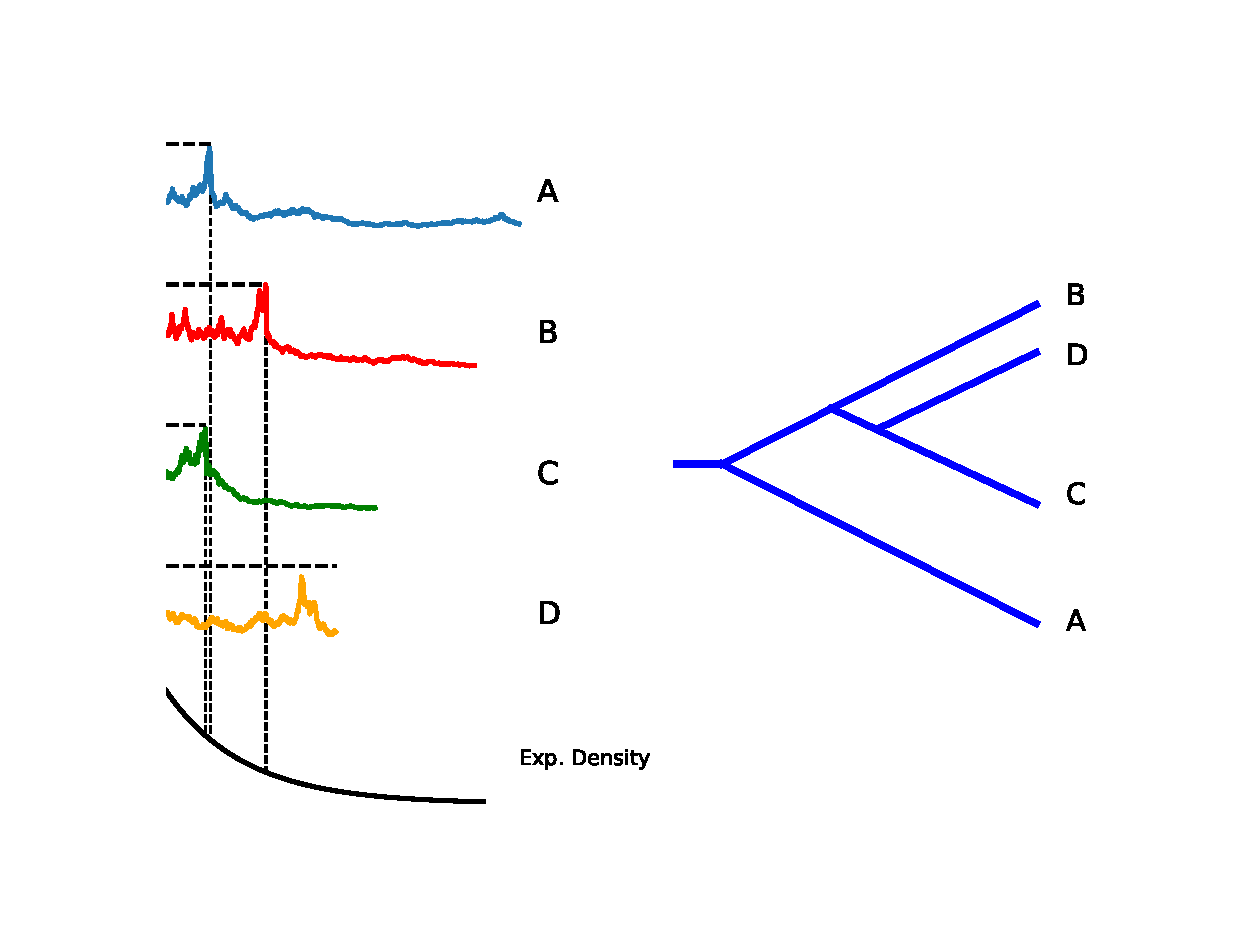
\includegraphics[width=\textwidth]{AncillaryFiles//figure3.eps}
\caption{An illustration of the formation of a phylogenetic tree. The left-hand side of the figure denotes times at which the barrier is hit, triggering mass migrations. Note that the length of the tree corresponds with the length of the path starting at $A$, which is also the same as the sums of the other branches.} \label{evo1}
\end{center} 
\end{figure}


\section{Computational Algorithm}

In previous sections, we have described how oftentimes there are multiple routes that are possible when a particular point of origin is posited. Here I show how one can couple choice of the optimal path through a tree by working recursively back through the tree, employing a dynamic programming algorithm to obtain the probability that all points in the tree were the geographic point of origin of the tree. First, imagine that all interior nodes have been enumerated in depth-first order, so that nodes nearer to leaves or taxa carry lower indices. This allows a backwards traversal of the tree via the index. 

Label each location along the tree as  $l=1,2,3,\hdots,L$, and the interior nodes (deeper nodes are lower numbers) as $k=1,2,3,\hdots K$. 

We can now recursively develop an expression for the probability that location $i$ is the origin after having traversed the $k$th node. We will begin by treating the case in which branch lengths are known, as the case in which they are not known can be handled by appropriate normalization of branch lengths. 

Let $P^*_{i,k}$ denote the likelihood that $i$ is the point of origin after considering the subtree spanned by node $k$. Let $t_{ik}$ denote the length of a chain starting at $k$ and moving on from $i$, and let $\delta_{ik}$ denote a dummy variable for whether or not any other chains have started from node $i$.   

At $k=0$, which is at the start of the algorithm, we start with $P_{i,0} =1$, $t_{i,0}=t_i$, and $n_i = 0$, and $\delta_{i,0}=0$. Define the children of a node as $A_k$ and define $A_{k,-i}$ as all the ancestors of node excepting ancestor $i$. Along with numbering the interior branches from $k$, we also attach $k$ to the interior branches of the tree leading into the node. 
Now, we are in a position to describe how the algorithm works. 

\begin{equation} \label{ca1}
\ln\left[ P^*_{i,k}\right]=\max_{j \in J_{ik}}\{{(\ln \left[f(n_j+1,t_j+t_{ij})\right]\delta_i+(1-\delta_i)\ln \left[P^*_{i,k-1}\right]\}
\end{equation}
subject to:
\begin{equation*}
s_t, \delta_t = 
\end{equation*}

\subsection{An example}



\section{Extensions}

\subsection{Approximations}

Using Stirling's approximation, one can write the likelihood very simply, which relates the jump method to simple counting. 


\subsection{Expanded likelihoods}
There are many ways in which the model can be extended. As alluded to above, when equipped with a model producing a likelihood, one can bind this to other components of a likelihood. 

For example, one possible idea is to interpret the likelihood presented in the previous few pages as a conditional likelihood, and incorporate it into a joint estimation procedure. For example, if one has a means of computing the likelihood of a particular tree, one can then think about the joint distribution of a likelihood and a tree at the same time using the simple probabilistic relationship:
$$
P(\mathcal{T},\mathcal{H})=P(\mathcal{H}|\mathcal{T})P(\mathcal{T})
$$
This is important because th
ere are so many methods for computing the likelihood of a given linguistic tree. This allows one to consider a migratory route as part of the estimation process, rather than just something loosely implied by the structure of the tree. One can also form a picture of the distribution of trees and roots once one is equipped with a likelihood function. 

Another important facet is the ability to include information for other sources, as in a Bayesian analysis. 

\subsection{Including additional information about migrations}

Part of the optimization relationship can also include additional information about what routes are more likely. As one example, one might include a matrix of physical distances or travel costs between points. This matrix might even reflect.\footnote{If one is interested, computational algorithms and extensions can be found on the project site:} 

\section{Applications}


\section{Appendix}
In the following I demonstrate an application of the algorithm in calculating the likelihood of a more complex tree. A Python implementation of the algorithm, along with some supporting materials, can be found on the project website. The following presents a detailed application of how to calculate the (concentrated) likelihood that any given location is the point of origin of the linguistic stock. 




\newpage
\bibliographystyle{apalike}
\bibliography{bibfile}

\end{document} 
